\newpage
\section{Задание 3 --- Нарисовать картинку}

Вариант №2.

\begin{itemize}
\item{Первая картинка}

  \begin{center}
    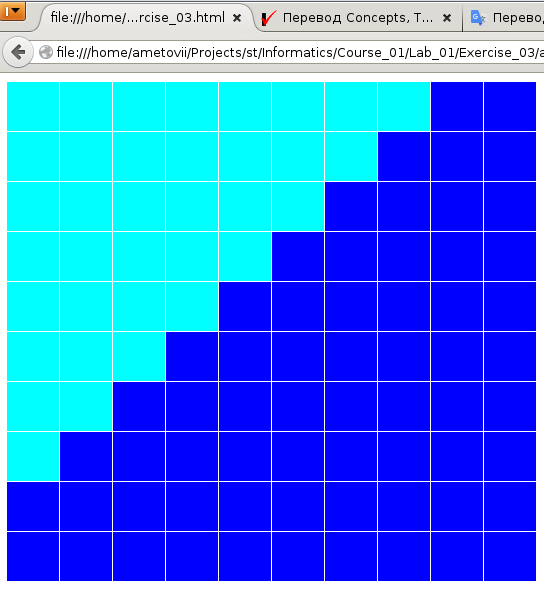
\includegraphics[width=9cm]{img/exercise_03/a/01.png}
  \end{center}

  Исходный код \verb|exercise_03.html|:
\begin{verbatim}
<head>
  <link rel=stylesheet type="text/css" href="1.css">
</head>
<body>
  <script>
    var n=10; var s;
    document.write("<table>");

      for (i=1; i<=n; i=i+1)
      {
       document.write("<tr>")

       for (j=1; j<=n; j=j+1)
       {
     
        if (j>(9-i)) s="class='r2'";
        else s="class='r1'";
        document.write("<td "+s+"> </td>");
       }
       document.write("</tr>");
      }
      document.write("</table>");
  </script>
</body>
\end{verbatim}

Исходный код \verb|1.css|:

\begin{verbatim}
table { border-collapse:collapse;}
td    {width: 50px; height: 50px; border: 1px solid white;}
.r1   {background-color: cyan;}
.r2   {background-color: blue;}
\end{verbatim}

\item{Вторая картинка}

  \begin{center}
    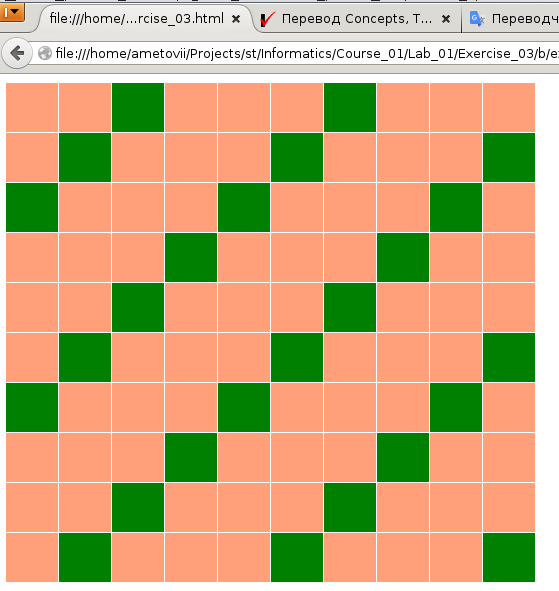
\includegraphics[width=9cm]{img/exercise_03/b/01.png}
  \end{center}

  Исходный код \verb|exercise_03.html|:

\begin{verbatim}
<head>
  <link rel=stylesheet type="text/css" href="1.css">
</head>
<body>
  <script>
    var n=10; var s;
    document.write("<table>");

      for (i=1; i<=n; i=i+1)
      {
       document.write("<tr>")

       for (j=1; j<=n; j=j+1)
       {
     
        if (((j+i)%4) == 0) s="class='r2'";
        else s="class='r1'";
        document.write("<td "+s+"> </td>");
       }
       document.write("</tr>");
      }
      document.write("</table>");
  </script>
</body>
\end{verbatim}

Исходный код \verb|1.css|:

\begin{verbatim}
table { border-collapse:collapse;}
td    {width: 50px; height: 50px; border: 1px solid white;}
.r1   {background-color: LightSalmon;}
.r2   {background-color: green;}
\end{verbatim}
\end{itemize}
